\documentclass[a4paper,12pt]{article}
\usepackage{hieroglf} % 添加古埃及象形文字
\usepackage{pifont} % 添加 Dingbat
\usepackage{tikz} % 添加绘图

\usepackage[top=1in,bottom=1in,left=1in,right=1in]{geometry} % 用于设置页面布局
\usepackage{xeCJK} % 用于使用本地字体
\usepackage[super, square, sort&compress]{natbib} % 处理参考文献
\usepackage{titlesec, titletoc} % 设置章节标题及页眉页脚
%\usepackage{xCJKnumb} % 中英文数字转换
\usepackage{amssymb}
\usepackage{amsmath} % 在公式中用\text{文本}输入中文
\usepackage{diagbox}
\usepackage{multirow} % 表格中使用多行
\usepackage{booktabs} % 表格中使用\toprule等命令
\usepackage{rotating} % 使用sidewaystable环境旋转表格
\usepackage{tabularx}
\usepackage{graphicx} % 处理图片
\usepackage{footnote} % 增强的脚注功能,可添加表格脚注
\usepackage{threeparttable} % 添加真正的表格脚注,示例见README
\usepackage{hyperref} % 添加pdf书签

\usepackage{tikz}
\usetikzlibrary{shapes,arrows,shadows}

% 字体设置
\setmainfont{Times New Roman}
\setsansfont[Scale=MatchLowercase,Mapping=tex-text]{PT Sans}
\setmonofont[Scale=MatchLowercase]{PT Mono}
\setCJKmainfont[ItalicFont={Kaiti SC}, BoldFont={Heiti SC}]{Songti SC}
\setCJKsansfont{Heiti SC}
\setCJKmonofont{Songti SC}
% \setCJKmainfont[BoldFont={FZXiaoBiaoSong-B05S}]{Songti SC}
% \setCJKfamilyfont{kai}[BoldFont=Heiti SC]{Kaiti SC}
% \setCJKfamilyfont{song}[BoldFont=Heiti SC]{Songti SC}
% \setCJKfamilyfont{hei}[BoldFont=Heiti SC]{Heiti SC}
% \setCJKfamilyfont{fsong}[BoldFont=Heiti SC]{Songti SC}
% \newcommand{\kai}[1]{{\CJKfamily{kai}#1}}
% \newcommand{\hei}[1]{{\CJKfamily{hei}#1}}
% \setromanfont[Mapping=tex-text]{TeXGyrePagella}
% \setsansfont[Scale=MatchLowercase,Mapping=tex-text]{TeXGyrePagella}
% \setmonofont[Scale=MatchLowercase]{Courier New}
%%设置常用中文字号,方便调用
\newcommand{\erhao}{\fontsize{22pt}{\baselineskip}\selectfont}
\newcommand{\xiaoerhao}{\fontsize{18pt}{\baselineskip}\selectfont}
\newcommand{\sanhao}{\fontsize{16pt}{\baselineskip}\selectfont}
\newcommand{\xiaosanhao}{\fontsize{15pt}{\baselineskip}\selectfont}
\newcommand{\sihao}{\fontsize{14pt}{\baselineskip}\selectfont}
\newcommand{\xiaosihao}{\fontsize{12pt}{\baselineskip}\selectfont}
\newcommand{\wuhao}{\fontsize{10.5pt}{\baselineskip}\selectfont}
\newcommand{\xiaowuhao}{\fontsize{9pt}{\baselineskip}\selectfont}
\newcommand{\liuhao}{\fontsize{7.5pt}{\baselineskip}\selectfont}

% 章节标题显示方式及页眉页脚设置
% \item xCJKnumb是自己额外安装的包
% \item titleformat命令定义标题的形式
% \item titlespacing定义标题距左、上、下的距离
\titleformat{\section}{\raggedright\large\bfseries}{\thesection}{1em}{}
\titleformat{\subsection}{\raggedright\normalsize\bfseries}{\thesubsection}{1em}{}
\titlespacing{\section}{0pt}{*0}{*2}
\titlespacing{\subsection}{0pt}{*0}{*1}
% 由于默认的2em缩进不够,所以我手动调整了,但是在windows下似乎2.2就差不多了,或者是article中没有这个问题
\setlength{\parindent}{2.2em}

% 设置表格标题前后间距
\setlength{\abovecaptionskip}{0pt}
\setlength{\belowcaptionskip}{0pt}


\renewcommand{\refname}{\bfseries{参~考~文~献}} %将Reference改为参考文献(用于 article)
% \renewcommand{\bibname}{参~考~文~献} %将bibiography改为参考文献(用于 book)
\renewcommand{\baselinestretch}{1.38} %设置行间距
\renewcommand{\figurename}{\small\ttfamily 图}
\renewcommand{\tablename}{\small\ttfamily 表}


\newcommand{\specialcell}[2][c]{%
  \begin{tabular}[#1]{@{}c@{}}#2\end{tabular}}

\pmhgfamily

\title{关于知识表示和演化的几何化构想}
\author{苑明理}
\date{2015年12月}

\begin{document}

\maketitle{}

\renewcommand\contentsname{目录}
\setcounter{tocdepth}{2}
\tableofcontents

\newpage

\section{前言}

人类的知识之旅充满了挑战。不论琢磨推敲式的守成,或者另辟蹊径的创新,点滴的进步日积月累方才筑成知识的殿堂。
承载着人们对特定对象的认知,知识都是藉由一定的形式来表达的。面对复杂的事物,人们甚至发展出多种表示方法,
从不同侧面折射事物本来的面目。不断的推陈出新,让知识的考掘变成一件有意义的事情。

然而,能否有一个数学化的方法来描述知识的演进呢?知识的演进能否在事前给予适当的预测呢?
本文尝试提出一种几何化的研究思路来回答这个问题。

我们首先会回顾科学史上的两个例子—古老的数制的形成和最近一百年间理论物理的发展,并由此引申出两个问题—知识的最优表示问题和演化问题。
然后参照数制的例子,我们会尝试在几何化的前提下,把最优表示问题和演化问题联系起来,由此形成我们对知识演化的一个理论框架。

任何理论的假设必须经由实际数据的检验,因此有三个问题需要解决:
\begin{itemize}
\item 构造合理的实测数据集
\item 从实测数据反推几何构形的方法
\item 验证我们的假设—最优表示和演化之间联系—的方法
\end{itemize}

本文作为一个研究提议,仅仅将这样三个问题提出来,作为进一步研究的起点.

\newpage

\section{科学史的回顾}

\subsection{数制的历史}

大约在 18000 ~ 20000 BC 的 Ishango 骨刻,是目前人们发现的最早和数目有关的考古实物,它处在刻痕记事的阶段。
如果不考虑实物的形态,仅从抽象角度看,在这个阶段人们采用符号 1 的累记来表示更大的数目。
这种方式在表示形式上极为繁赘,尤其对大的数目,几乎不具有实际的可行性。但凭借这种简单的记号,人们有了对数目概念的理解。

\begin{figure}[ht]
\centering
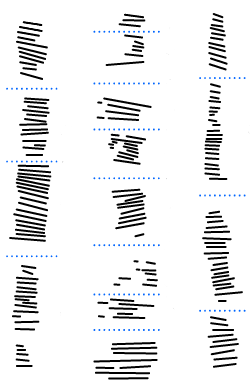
\includegraphics[width=1.5in]{images/IshangoAllColumns.png}
\caption{Ishango 骨刻(图片来自于维基共享资源计划)}
\end{figure}

在这个阶段,人们可以通过分堆的方法进行乘法运算。但这种方法仅仅限于小数目之间的乘法。

\begin{table}[tbhp]
\centering
\begin{tabular}{|c|c|c|c|c|}
\hline
\specialcell{ \ding{108} \\ \ding{108}\ding{108} } &
\specialcell{ \ding{108} \\ \ding{108}\ding{108} } &
\specialcell{ \ding{108} \\ \ding{108}\ding{108} } &
\specialcell{ \ding{108} \\ \ding{108}\ding{108} } &
\specialcell{ \ding{108} \\ \ding{108}\ding{108} } \\
\hline
\end{tabular}
\caption{计算 3 与 5 的乘积}
\end{table}

人类进入文明以后,有了对抽象符号更强的操作能力。在古埃及,人们发明了另外一种复杂的计数体系,它能表示整数、分数和相关运算。
我们这里仅仅简单展示整数的表示和乘法运算。

\begin{table}[tbhp]
\centering
\begin{tabular}{|c|ccccccc|}
\hline
数值 & 一 & 十 & 百 & 千 & 万 & 十万 & 百万 \\
符号 & \pmglyph{\Hone} & \pmglyph{\Hten} & \pmglyph{\Hhundred} & \pmglyph{\Hthousand} & \pmglyph{\HXthousand} & \pmglyph{\HCthousand} & \pmglyph{\Hmillion} \\
描述 & 单竖线 & 踵骨 & 绳圈 & 水莲 & 屈指 & 蝌蚪 & Heh 神\\
\hline
\end{tabular}
\caption{古埃及象形文字里的整数符号}
\end{table}

组合上述的基本符号,古埃及人可以表达一些相对较大的整数。但古埃及人组合这些符号的方式,并没有非常严格的方法:
既可以从左向右,也可以从右向左,有时也会竖写。除此以外,古埃及人做乘法的方式,更加显示出他们的数制还处于一种早期形态。
下图展示了古埃及人如何计算 11 与 35 乘积的过程。

\begin{figure}[ht]
\centering
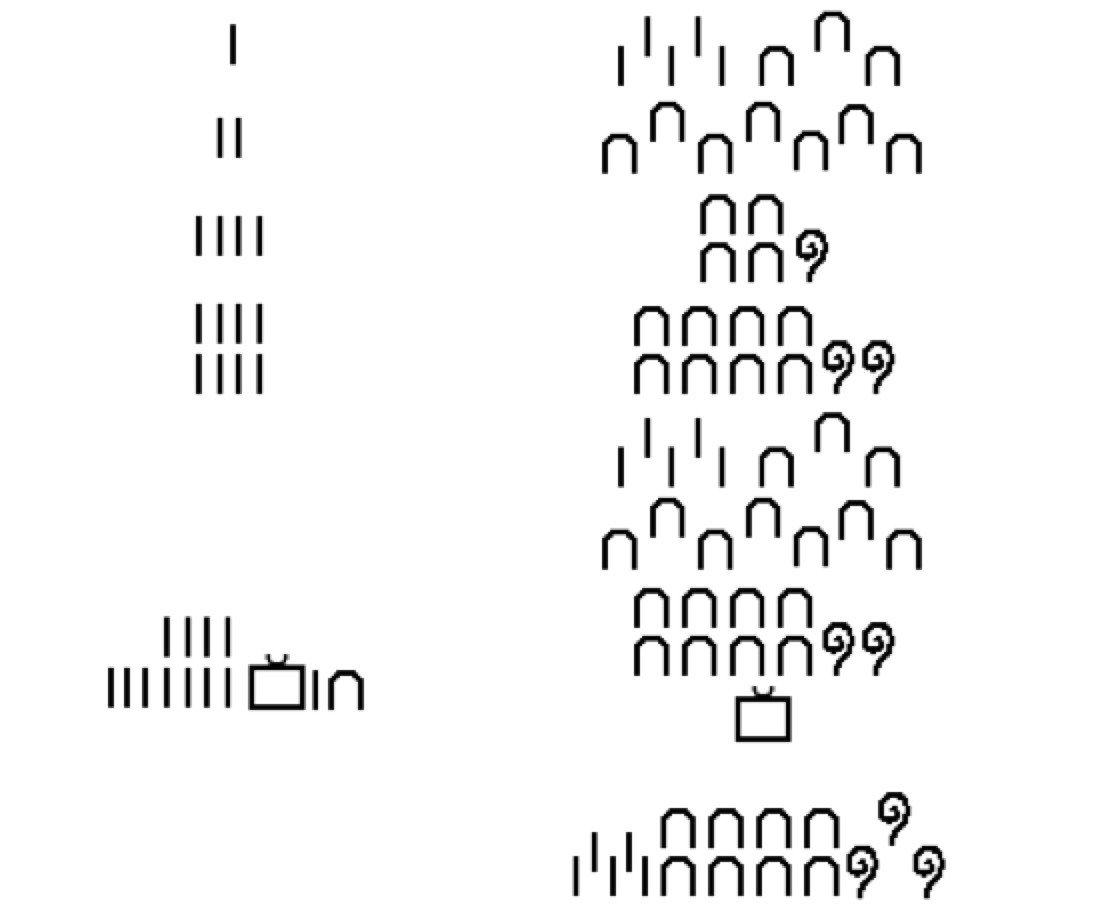
\includegraphics[width=3.5in]{images/ancient_egypt_multiplication.jpg}
\caption{计算 11 与 35 乘积}
\end{figure}

在这种方法里,首先构造 2 的幂的序列1、2、4、8……,同时 35 也按照 2 倍的关系相应扩大。
然后可以看出,11 能被分解成为了 1、2、8 的和,所以只要把 35 倍数里的 35、70、280 累加就可以得到结果。

但是数制的更加成熟的形态是数位制。在许多古文明中,数位制都被发明出来,如古巴比伦的 60 进制系统、古印第安文明的 20 进制系统。
对于乘法运算,中国古代很早就发明了九九乘法表,清华简中的“算表”作为考古实物依据,把发明年代至少向前推进到战国时代。
十进数位制和九九乘法表结合在一起,人们能够完整的表达所有自然数,并计算任意自然数的乘法。
当今,阿拉伯数字符号、十进数位制、九九乘法表都作为基础教育的内容,成为全人类分享的文明成果。

\begin{table}[tbhp]
\centering
\begin{tabular}{cccccccccccccccccccccccccccccccccccc}
  &   &   &   &   &   &   &   & 2 & 3 & 9 & 5 & 8 & 2 & 3 & 3\\
× &   &   &   &   &   &   &   &   &   &   &   & 5 & 8 & 3 & 0\\
\hline
  &   &   &   &   &   &   &   & 0 & 0 & 0 & 0 & 0 & 0 & 0 & 0\\
  &   &   &   &   &   &   & 7 & 1 & 8 & 7 & 4 & 6 & 9 & 9 &  \\
  &   &   &   &   & 1 & 9 & 1 & 6 & 6 & 5 & 8 & 6 & 4 &   &  \\
  &   & + &   & 1 & 1 & 9 & 7 & 9 & 1 & 1 & 6 & 5 &   &   &  \\
\hline
  &   &   &   & 1 & 3 & 9 & 6 & 7 & 6 & 4 & 9 & 8 & 3 & 9 & 0\\
\end{tabular}
\caption{竖式乘法的例子}
\end{table}

\subsection{理论物理百年}

1900年 Max Planck 通过对不完美的黑体辐射的 Wien 公式与 Rayleigh 公式的插值得到了 Planck 公式,给出了黑体辐射问题的一个数学描述。
在寻求 Planck 公式的理论说明的时候,Planck 引入了量子的概念,由此揭开了量子理论的序幕。

1905年是物理学的奇迹之年,在这一年 Albert Einstein 发表了四篇基础性的论文:
扩展了 Max Planck 的量子观点,提出光量子,解释了光电效应;研究了布朗运动,论证了原子的存在性;
发表了狭义相对论,在相对性原理的基础上揭示了一种新的时空观;同时,也提出了意义深远的质能等当关系。

1907年,Einstein 应用量子的概念解释了金钢石、石墨、硼和硅的室温摩尔热容比。1912年 Peter Debye 发展出了低温热容的量子理论。
1913年,玻尔应用量子的概念解释了氢原子光谱,成为老量子论的典范之作。

1915年 Albert Einstein 发表了广义相对论,基于更一般的相对性原理把引力几何化,用时空的弯曲来表达引力。

1918年,玻尔对应原理

1924年
1925年
1926年
1927年

经过1927年、1930年、1933年三次索尔维会议的论战,1935年 EPR 提出量子纠缠的概念

1935年 ER

1997年 Maldancena 发表 AdS/CFT

2010年 Van Raamsdonk 的几何—纠缠关系

2012年 Swingle 张量网络

2012年 Daniel Harlow和 John Preskill 量子纠错码与 AdS/CFT 的关系

2013年 Maldancena 和 Leonard Susskind 发表 ER = EPR 的猜想

\newpage

\section{研究思路概述}

\subsection{知识表示的几何化}

词嵌入模型揭开了知识表示的一种几何化思路,它提出的正则性因为保留了代数运算的优良性质,使得人们看到了这个模型的潜力。
然而,平直的高维向量空间是否是一个知识表示的恰当几何载体呢?这还是一个疑问。

举一个简单的例子:人物 $a$ 和 $b$ 之间有配偶关系 $R$,我们可以用下式表达:

\begin{equation}
R(a) = b
\end{equation}

并且很容易看到:

\begin{equation}
R(R(a)) = a
\end{equation}

即有如下公式: 

\begin{equation}
R^2 = I
\end{equation}

此处 $I$ 是恒同变换。公式(3)里的 $R$ 很难用一个向量来表示,却很容易用一个 $S_1$ 上的角度为 $\pi$ 的旋转来表示。

这给我们一定的提示,或许我们可以从普通的欧式空间扩展到更一般的流形上,而且这个流形上可以保留良好的代数结构。
我们会在第 \ref{sec:geometry} 节详细讨论这个几何化方案,并以数制作为几何化的例子。
而且通过例子,我们可以建立一个翻译表,把日常语言里描述知识的词汇对应到几何构形上。

\subsection{最优表示问题}

\subsection{演化问题}

\subsection{两个问题之间的联系}

\newpage

\section{概念网络的几何化}
\label{sec:geometry}

\newpage

\section{最优表示问题}

\newpage

\section{演化问题}

\begin{tikzpicture}[scale=0.03125]
  \draw          (  0, 256)
              -- (512, 256);
  \draw[fill]    ( 16, 256) circle [radius=1] node [above] {$-4$};
  \draw[fill]    ( 32, 256) circle [radius=1] node [above right] {$-3$};
  \draw[fill]    ( 64, 256) circle [radius=1] node [above right] {$-2$};
  \draw[fill]    (128, 256) circle [radius=1] node [above right] {$-1$};
  \draw[fill]    (256, 256) circle [radius=1] node [above right] {$0$};
  \draw[fill]    (384, 256) circle [radius=1] node [above left] {$+1$};
  \draw[fill]    (448, 256) circle [radius=1] node [above left] {$+2$};
  \draw[fill]    (480, 256) circle [radius=1] node [above left] {$+3$};
  \draw[fill]    (496, 256) circle [radius=1] node [above] {$+4$};

  \draw          (256,   0)
              -- (256, 512);
  \draw[fill]    (256,  16) circle [radius=1] node [above right] {$0$};
  \draw[fill]    (256,  32) circle [radius=1] node [above right] {$0$};
  \draw[fill]    (256,  64) circle [radius=1] node [above right] {$0$};
  \draw[fill]    (256, 128) circle [radius=1] node [above right] {$0$};
  \draw[fill]    (256, 256) circle [radius=1] node [above right] {$0$};
  \draw[fill]    (256, 384) circle [radius=1] node [above right] {$0$};
  \draw[fill]    (256, 448) circle [radius=1] node [above right] {$0$};
  \draw[fill]    (256, 480) circle [radius=1] node [above right] {$0$};
  \draw[fill]    (256, 496) circle [radius=1] node [above right] {$0$};

  \draw          (128, 128)
              -- (384, 128);
  \draw[fill]    (144, 128) circle [radius=1] node [above] {$-3$};
  \draw[fill]    (160, 128) circle [radius=1] node [above right] {$-2$};
  \draw[fill]    (192, 128) circle [radius=1] node [above right] {$-1$};
  \draw[fill]    (256, 128) circle [radius=1] node [above right] {$0$};
  \draw[fill]    (320, 128) circle [radius=1] node [above left] {$+1$};
  \draw[fill]    (352, 128) circle [radius=1] node [above left] {$+2$};
  \draw[fill]    (368, 128) circle [radius=1] node [above] {$+3$};

  \draw    (128, 384)
        -- (384, 384);
  \draw[fill]    (144, 384) circle [radius=1] node [below] {$-3$};
  \draw[fill]    (160, 384) circle [radius=1] node [below right] {$-2$};
  \draw[fill]    (192, 384) circle [radius=1] node [below right] {$-1$};
  \draw[fill]    (256, 384) circle [radius=1] node [below right] {$0$};
  \draw[fill]    (320, 384) circle [radius=1] node [below left] {$1$};
  \draw[fill]    (352, 384) circle [radius=1] node [below left] {$2$};
  \draw[fill]    (368, 384) circle [radius=1] node [below] {$3$};

  \draw          (128, 128)
              -- (128, 384);
  \draw[fill]    (128, 144) circle [radius=1] node [left] {$-8$};
  \draw[fill]    (128, 160) circle [radius=1] node [above left] {$-4$};
  \draw[fill]    (128, 192) circle [radius=1] node [above left] {$-2$};
  \draw[fill]    (128, 256) circle [radius=1];
  \draw[fill]    (128, 320) circle [radius=1] node [below left] {$-1/2$};
  \draw[fill]    (128, 352) circle [radius=1] node [below left] {$-1/4$};
  \draw[fill]    (128, 368) circle [radius=1] node [left] {$-1/8$};

  \draw          (384, 128)
              -- (384, 384);
  \draw[fill]    (384, 144) circle [radius=1] node [right] {$+1/8$};
  \draw[fill]    (384, 160) circle [radius=1] node [above right] {$+1/4$};
  \draw[fill]    (384, 192) circle [radius=1] node [above right] {$+1/2$};
  \draw[fill]    (384, 256) circle [radius=1];
  \draw[fill]    (384, 320) circle [radius=1] node [below right] {$+2$};
  \draw[fill]    (384, 352) circle [radius=1] node [below right] {$+4$};
  \draw[fill]    (384, 368) circle [radius=1] node [right] {$+8$};

  \draw [red, dashed, very thick]
           (  0, 256)
        -- (256,   0)
        -- (512, 256)
        -- (256, 512)
        -- cycle;

\end{tikzpicture}

\end{document}
